% Este archivo es parte de la memoria del proyecto fin de carrera
% de Manuel López Urbina. Protegida bajo la licencia GFDL.
% Para más información, la licencia completa viene incluida en el
% fichero fdl-1.3.tex

% Copyright (C) 2012 Manuel López Urbina

\chapter{Herramientas utilizadas}
\label{chap:herramientas} 

El presente capítulo recoge información acerca de las diferentes herramientas, tanto hardware como software, utilizadas durante el desarrollo del proyecto y para su posterior utilización. 

\section {Herramientas software}

El proyecto ha sido realizado haciendo uso del lenguaje de programación C y C++ junto con el uso de diversas bibliotecas. A continuación se realiza una breve descripción de cada una de ellas:

\begin{description} 

\item [OpenCV]
Es una biblioteca libre de visión artificial originalmente desarrollada por Intel. Desde la salida de su primera versión alfa en el mes de enero de 1999, se ha utilizado en infinidad de aplicaciones. Desde sistemas de seguridad con detección de movimiento, hasta aplicaciones para de control de procesos donde es requerido el reconocimiento de objetos. Esto es debido se publica bajo licencia BSD, permitiendo su utilización para propósitos comerciales y de investigación con las condiciones en ella expresadas.

OpenCV es multiplataforma, existiendo versiones para GNU/Linux, Mac OS X y Windows. Contiene más de 500 funciones que abarcan una gran gama de áreas en el proceso de visión, como reconocimiento de objetos (reconocimiento facial), calibración de cámaras, visión estereo y visión robótica.

El proyecto pretende proporcionar un entorno de desarrollo fácil de utilizar y altamente eficiente. Esto se ha logrado, realizando su programación en código C y C++ optimizados, aprovechando además las capacidades que proveen los procesadores multinúcleo, que como se verá en la presente memoria, su alta eficiencia, ha sido uno de los motivos principales para la elección de esta biblioteca.

\begin{figure}[H]
  \begin{center}
    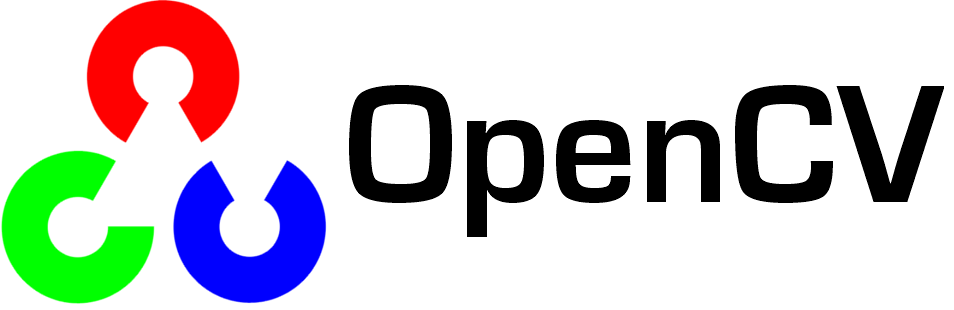
\includegraphics[scale=1]{opencv-logo.png}
  \end{center}
  \caption{Logotipo de OpenCV}
  \label{SRV-1}
\end{figure}

\item [Qt] es una biblioteca multiplataforma ampliamente utilizada para el desarrollo de aplicaciones con una interfaz gráfica de usuario, también es usado para el desarrollo de programas sin interfaz gráfica como herramientas para la línea de comandos y consolas para servidores.

Qt utiliza el estándar C++, pero hace un amplio uso de un generador de código especial (llamado compilador Meta Object, o MOC), junto con varias macros para enriquecer el lenguaje. Qt también puede ser usado con otros lenguajes de programación a través de enlaces al lenguaje. Permite su ejecución en las principales plataformas de escritorio y algunas plataformas móviles. También es usado en sistemas informáticos empotrados para automoción, aeronavegación y aparatos domésticos como frigoríficos.

Distribuido bajo los términos de la licencia GNU (entre otras), Qt es software libre y de código abierto. Todas las ediciones soportan el compilador GCC y la suite de Visual Studio entre otros.

\begin{figure}[H]
  \begin{center}
    
\includegraphics[scale=0.3]{qt-logo.jpg}
  \end{center}
  \caption{Logotipo de Qt}
  \label{SRV-1}
\end{figure}

\item [Surveyor Robot Software] software desarrollado por John Cummins junto con los agentes de laboratorio de la Universidad de Brooklyn con la asistencia de M.P. Azhar, y la supervisión del profesor Sklar empleando el lenguaje de programación C++ para el control del vehículo SRV-1 Surveyor. El código está liberado bajo Copyleft.

\item [Simple DirectMedia Layer (SDL)] es un conjunto de bibliotecas desarrolladas en el lenguaje de programación C. Proporciona las funciones básicas para la realización de operaciones de dibujo en dos dimensiones, gestión de efectos de sonido y música, además de carga y gestión de imágenes. Fueron desarrolladas inicialmente por Sam Lantinga, un desarrollador de videojuegos para la plataforma GNU/Linux.

Pese a estar programado en C, tiene wrappers a otros lenguajes de programación como C++, Ada, C\#, BASIC, Erlang, Lua, Java, Python, etc. También proporciona herramientas para el desarrollo de videojuegos y aplicaciones multimedia. Una de sus grandes virtudes es el tratarse de una biblioteca multiplataforma, siendo compatible oficialmente con los sistemas Microsoft Windows, GNU/Linux, Mac OS y QNX, además de otras arquitecturas y sistemas como Sega Dreamcast, GP32, GP2X, etc.
La biblioteca se distribuye bajo la licencia LGPL, que es la que ha provocado el gran avance y evolución de SDL.

\begin{figure}[H]
  \begin{center}
    
\includegraphics[scale=0.3]{sdl-logo.png}
  \end{center}
  \caption{Logotipo de SDL}
  \label{SRV-1}
\end{figure}
\item [Qt Creator] es un IDE creado por Trolltech para el desarrollo de aplicaciones con las bibliotecas Qt.

\begin{figure}[H]
  \begin{center}
    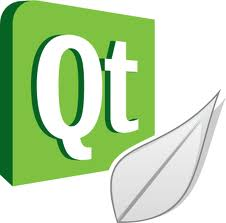
\includegraphics[scale=0.3]{qtcreator-logo.jpg}
  \end{center}
  \caption{Logotipo de Qt Creator}
  \label{SRV-1}
\end{figure}

\end{description}

\subsection{Licencia}

La aplicación OpenTSR es software libre: usted puede redistribuirlo y / o modificar bajo los términos de la Licencia Pública General de GNU según lo publicado por la Free Software Foundation, ya sea la versión 3 de la Licencia, o (a su elección) cualquier versión posterior.\\

Este programa se distribuye con la esperanza de que sea útil, pero SIN NINGUNA GARANTÍA, incluso sin la garantía implícita de COMERCIALIZACIÓN o IDONEIDAD PARA UN PROPÓSITO PARTICULAR. Ver el GNU General Public License para más detalles. Debería haber recibido una copia de la Licencia Pública General de GNU junto con este documento. Si no es así, consulte \href{http://www.gnu.org/licenses}{GNU Licenses}.

\section{Herramientas hardware}

La figura \ref{figura:elementos-hardware-empleados} nos proporciona una visión general de los diferentes elementos hardware empleados en el desarrollo del proyecto. En los sucesivos puntos se enumeran las características de cada uno de ellos.\\

\begin{figure}[H]
  \begin{center}
    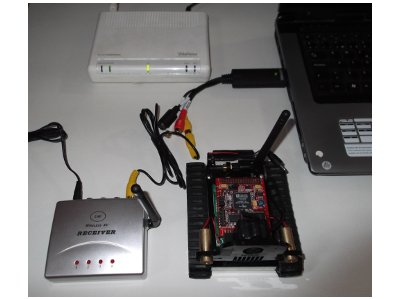
\includegraphics[scale=0.8]{elementos-hardware.jpg}
  \end{center}
  \caption{Imagen de los diferentes elementos hardware empleados.}
  \label{figura:elementos-hardware-empleados}
\end{figure}

\subsection{Vehículo SRV-1}

El elemento hardware principal utilizado es el vehículo \emph{Surveyor SRV-1 WiFi webcam robot}. Dicho vehículo ha sido diseñado para la investigación, la educación, y la exploración, Surveyor SRV-1 es robot que cabe en la palma de la mano, puede desplazarse por superficies lisas y rugosas gracias a sus ruedas tipo tanque fabricadas con caucho. \\

El robot SRV-1 incorpora un potente procesador a 500 MHz denominado Blackfin BF537 con 32 MB de RAM y 4 MB de memoria Flash. Equipado con una cámara a color de resolución 1280x1024 (1,3 megapíxeles) y dos sensores láser que lo dotan de la capacidad de evitar obstáculos. La batería recargable de 7,2 V permite una autonomía de hasta 4 horas de duración y una placa de comunicación WLAN 802.11b/g para su seguimiento y control. \\

\begin{figure}[H]
  \begin{center}
    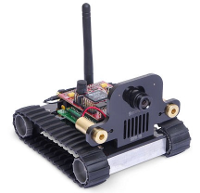
\includegraphics[scale=1]{srv-1.png}
  \end{center}
  \caption{Imagen del vehículo SRV-1}
  \label{SRV-1}
\end{figure}

\subsubsection{Características principales} 

\begin{itemize}
\item Diseño Open Source con acceso completo al código fuente (GPL) y esquemáticos. 
\item El robot es totalmente programable para su funcionamiento autónomo. 
\item Amplio soporte de software a través de aplicaciones de terceros. 
\item Posibilidad de conducir o teleoperar con el robot por medio del software proporcionado (consola java) o de forma remota a través de navegador web. 
\item El software del host es procesado en el servidor web junto con almacenamiento de vídeo en streaming.
\item El robot puede ejecutar programas escritos en C y almacenados en su memoria flash de a bordo. 
\item Control remoto inalámbrico con alcance de 100 metros en interiores y de hasta 1000m en aire libre (visión directa). 
\item El robot puede ser controlado desde un terminal o consola para las pruebas de fácil Linux 2.6 apoyo, así como "bare metal"de programación con GNU BFIN-elf-gcc 
\end{itemize}

\subsubsection{Características hardware} 

\begin{itemize}

\item \textbf{Procesador:} de 500 MHz y 1000 MIPS de nombre Blackfin BF537 con 32MB SDRAM y 4MB de memoria Flash. 

\item \textbf{Cámara:} 1,3 megapíxeles Omnivision OV9655 160x128 resolución de 1280x1024. 

\item \textbf{Placa de control:} Lantronix MatchPort 802.11b/g Wi-Fi 
\item \textbf{Alcance:} 100 metros en interiores, 1000m en situaciones de visión directa. 
\item \textbf{Sensores:} 2 punteros láser para mediciones y soporte para hasta 4 módulos Maxbotics ultrasónicos y varios sensores I2C. 
\item \textbf{Conjunto:} estilo tanque con tracción diferencial a través de cuatro motores reductores de precisión (reducción 100:1). 
\item \textbf{Velocidad:} 20 cm - 40 cm por segundo (aproximadamente 1 pie/seg o 0.5 millas/hora). 
\item \textbf{Chasis:} Aluminio mecanizado. 
\item \textbf{Dimensiones:} 120 mm largo x 100mm ancho x 80mm de altura (5" x 4"x 3"). 
\item \textbf{Peso:} 350gm (12 oz). 
\item \textbf{Potencia:} 7,2 V 2AH Li-poli batería - 4 + horas de autonomía por carga. 
\item \textbf{Cargador:} 100-240VAC 50/60Hz (enchufe de EE.UU.). 1.1.3. 
\end{itemize}

Debido a que el cargador posee el enchufe siguiendo el estándar americano ha sido necesario un conversor a formato europeo para realizar las cargas de la batería que incorpora el vehículo.

\subsubsection{Características software} 

\begin{itemize}

\item \textbf{Firmware del Robot:} fáciles de actualizar, escrito en lenguaje C bajo GPL Open Source, compilado con GNU BFIN-elf-gcc y cadenas de herramientas BFIN-gcc-uClinux. 

\item \textbf{Programación:} el vehículo dispone de un intérprete de lenguaje C con funciones específicas. 

\item \textbf {Comandos de control:} el robot proporciona una serie de comandos para la ejecución de movimientos programables por el usuario desde la memoria Flash de a bordo. 

\item \textbf{Herramientas de desarrollo:} a través de cadenas de herramientas GNU http://blackfin.uclinux.org. 

\item \textbf{Consola del programa:} aplicación basada en Java, funciona en Windows, Mac, Linux. 

\item \textbf {WebcamSat:} módulo de servidor web integrado en el software de la consola, permite que varios espectadores simultáneos remotos a través de Internet. 

\item \textbf{Protocolo de control de robot:} fácil de usar desde otras aplicaciones. 
\end{itemize}

En cuanto a software disponible proporcionado por terceros: 

\begin{itemize}

\item \textbf{RoboRealm:}  SRV-1 puede ser controlado directamente desde RoboRealm, un software basado en Windows con paquete específico para visión artificial en robots. Las extensiones para Robo-Realm SRV-1 permite la creación de guiones que combinan el procesamiento de imágenes de vídeo en vivo desde el robot, por ejemplo, filtrado de color, seguimiento, detección de bordes, extracción de características, y posterior procesamiento de la decisión y movimiento del robot, facilitando la creación de conductas tales como la localización de objetos y el rastreo, evasión de obstáculos, la detección de movimiento, notificación, etc, con una red interfaz, el control puede ser escrito en C / C++, Python, Java, C, Lisp, Visual Basic, WScript y COM a través de la API RoboRealm. 

\item \textbf{Microsoft Robotics Studio:}  Drivers para el SRV-1 de Microsoft Robotics Studio están disponibles. MSRS es un entorno basado en Windows para desarrolladores académicos, aficionados y comerciales para crear aplicaciones de robótica a través de una amplia variedad de hardware. 

\item \textbf{Webots:} Soporte SRV-1 incluido en Webots, es un software de simulación robótica móvil, proporciona un entorno de prototipado rápido para el modelado, la programación y simulación de robots móviles con sistema operativo Windows, Mac / X y Linux. El modelado en 3D y la física son excepcionales. 

\end{itemize}

Para más información acerca del vehículo robótico acceda a la web del \href{http://www.surveyor.com/SRV\_info.html}{sitio oficial}\footnote{Web del sitio oficial: \url{http://www.surveyor.com/SRV\_info.html}.}.

\subsection{Router}

Ha sido necesario disponer de un router para establecer una comunicación inalámbrica entre el ordenador y el vehículo SRV-1. Dicho vehículo posee la característica de realización de conexiones punto a punto o ad-hoc con el inconveniente de ser redes mucho más inestables. \\

Para solucionar el problema de la inestabilidad se ha optado por la creación de una infraestructura de red con la ayuda de un router proporcionando una mayor robustez a la conexión además de permitir incorporar más dispositivos a nuestra red en caso de que sea necesario. \\

\begin{figure}[H]
  \begin{center}
    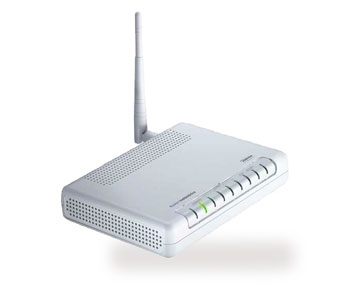
\includegraphics[scale=0.7]{router.png}
  \end{center}
  \caption{Imagen del router empleado.}
  \label{Imagen del router empleado}
\end{figure}

\subsection{Cámara, receptor inalámbrico y capturadora de vídeo}

Para la transmisión de vídeo desde el vehículo al ordenador, debido al estado defectuoso de la cámara incorporada en el vehículo SRV-1, ha sido necesario disponer de una cámara inalámbrica, un receptor inalámbrico para recoger las imágenes de la cámara y una capturadora de vídeo para digitalizarlas y visualizarla en el ordenador.

\subsubsection {Capturadora de vídeo}

El conversor analógico/digital o capturadora empleada es una König modelo CMP-USBVG. Sus características son las siguientes:
 
\begin{itemize}
\item Marca: König.
\item Modelo: CMP-USBVG5.
\item Resolución máxima: 720x480 Píxeles.
\item Sistemas operativos compatibles: Windows 2000/XP/Vista, drivers no oficiales para Linux.
\item Requisitos de energía: 5V.
\item Interfaz:	USB 2.0.
\item Velocidad de captura en vídeo digital: 30 fps.
\item Entrada de S-Video.
\item Entrada compuesta de vídeo.		
\end{itemize}

Consulte la sección \ref{sec:drivers-capturadora} correspondiente a la guía de usuario para acceder a las instrucciones para la instalación de los drivers de la capturadora.\\

\begin{figure}[H]
  \begin{center}
    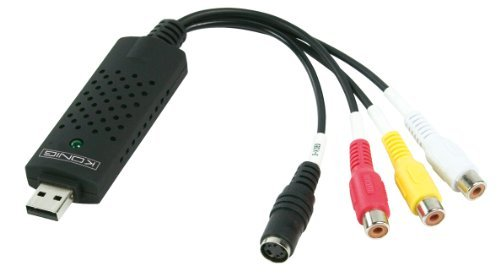
\includegraphics[scale=0.5]{capturadora.jpg}
  \end{center}
  \caption{Imagen de la capturadora o conversor analógico/digital.}
  \label{fig:capturadora}
\end{figure}

\subsubsection{Cámara y receptor inalámbrico} 

La minicámara utilizada está formada por un sensor 1/4'' OmniVision CMOS que ofrece una imagen a color, con una resolución de 380 líneas en TV. Posee un micrófono incorporado que hace que el audio se grabe junto al vídeo. La minicámara es capaz de captar imágenes donde la iluminación es baja siempre y cuando sea superior a 3.0 Lux lo que la hacen adecuada en situaciones de escasa luminosidad. Permite alimentación conectándola directamente a la red  eléctrica o bien usando una pila, gracias al clip de alimentación para pilas de 9V que incorpora.\\

La señal de vídeo y audio se transmite hasta el receptor atravesando paredes y muros. Dispone de una distancia máxima de utilización de 30 metros en situaciones de interior con obstáculos o de hasta 100 metros en exteriores.\\
 
El receptor inalámbrico tiene la posibilidad de recoger la señal de 4 minicámaras gracias a sus cuatro canales, los cuales están capacitados para recoger audio y vídeo por cada canal. Los canales se pueden seleccionar a través de un swich que se encuentra en la parte trasera del receptor. La salida del receptor permite su conexión hacia un videograbador, tarjeta capturadora o monitor mediante un cable RCA. Los canales tiene dos modalidades de visualización y/o grabación, bien mostrando de forma permanente un mismo canal o bien mostrando los cuatro canales de manera secuencial. La alimentación del receptor se hace mediante un alimentador de DC 8V/180 mA.\\

\begin{figure}[H]
  \begin{center}
    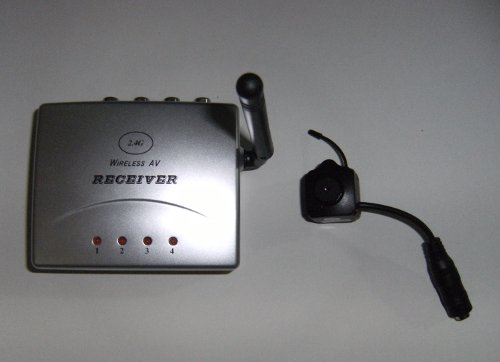
\includegraphics[scale=0.5]{receptor-y-camara.jpg}
  \end{center}
  \caption{Imagen de la cámara y el receptor inalámbricos.}
  \label{imagen-pad}
\end{figure}


\subsection{Gamepad}

Para dotar al vehículo sistema de un control más ergonómico y funcional se ha utilizado un mando con conexión USB como el que muestra la figura \ref{imagen-pad}.\\

\begin{figure}[H]
  \begin{center}
    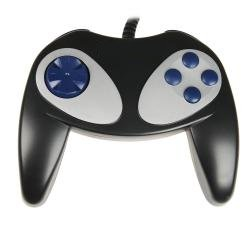
\includegraphics[scale=0.7]{pad.png}
  \end{center}
  \caption{Imagen del gamepad USB utilizado.}
  \label{imagen-pad}
\end{figure}

\subsection{Ordenador}

Por último ha sido necesario un ordenador portátil con un entrono GNU/Linux para la ejecución del software de control, el cual se encargará del procesamiento de las señales de vídeo y la transmisión de las respuestas al vehículo. La aplicación desarrollada también proporciona un medio para el manejo del vehículo por parte del usuario. Imprescindible que el ordenador incorpore de tarjeta WiFi inalámbrica.\\

